\section{Controller Switching Thresholds and Overall Tuning}
\label{sec:thresholds}

In and of itself, the switching PID controller described in section \ref{sec:idealcontroller} has five parameters; three controller gains plus the two switching thresholds.
Although all could likely be determined analytically or via simulation, the non-standard nature of the controller and reliance on external physical effects (see section \ref{sec:SimulationLimitations}) makes the process non-trivial.
As such, finding parameters and tuning was accomplished by applying a systematic experimental method.

Of critical importance is the threshold where the proportional controller is replaced by a PD controller.
Figure \ref{fig:threshold} below shows two plots of position vs. time as the truss moves from the pick-up position (0.79 rad = +45$^\circ$) to the drop position (-0.79 rads = -45$^\circ$) and back to initial position (0 rads). 
The blue plot represents a correctly calibrated controller that begins changing the truss direction at the drop position. 
As the truss decelerates, the red plot shows a measure of overshoot at 1.76s. 
This overshoot can be attributed to the switch from a P to PD controller occurring too \q{late}.
The condition used to determine when switching should occur is the error magnitude.
The overshoot can be corrected by increasing error magnitude at which a switch will happen.
It should be noted that different thresholds are used when the arm moves $45^\circ$ and when it moves $90^\circ$.
% 	More on why?


%In order to function optimally, the correct P, PD, and PID controller parameters must be properly determined for the specific system under consideration. 
%This was accomplished by applying a systematic experimental method. 
%The figure below shows two plots of position vs. time as the truss moves from the pick-up position (0.79 rad = +45 degrees) to the drop position (-0.79 rads = -45 degrees) and back to initial position (0 rads). 
%During the initial truss movement from pick-up to drop-off, a proportional control is applied, which was adjusted to produce a motor saturation at 10V. 
%As the truss decelerates, the red plot shows a measure of overshoot at 1.76s. 
%This overshoot, of approximately 0.35 rads, can be attributed to a PD control parameter that is too low. 
%By adjusting this parameter incrementally while continually running tests, an optimal value for PD that minimizes overshoot while avoiding over-damping, can be achieved. 
%The blue plot represents a correctly calibrated controller that begins changing the truss direction at the drop position. 
%Comparing the blue plot at 1.75s to the red plot in the range of 1.8s - 2s shows how the integral gain applied at the drop-off can be calibrated according to what will minimize the duration of oscillatory behaviour at low system velocities. 

%See figure \ref{fig:threshold}.

%TODO: Add figure (+ capture data) for threshold too high.

\begin{figure}[htp]
    \centering
    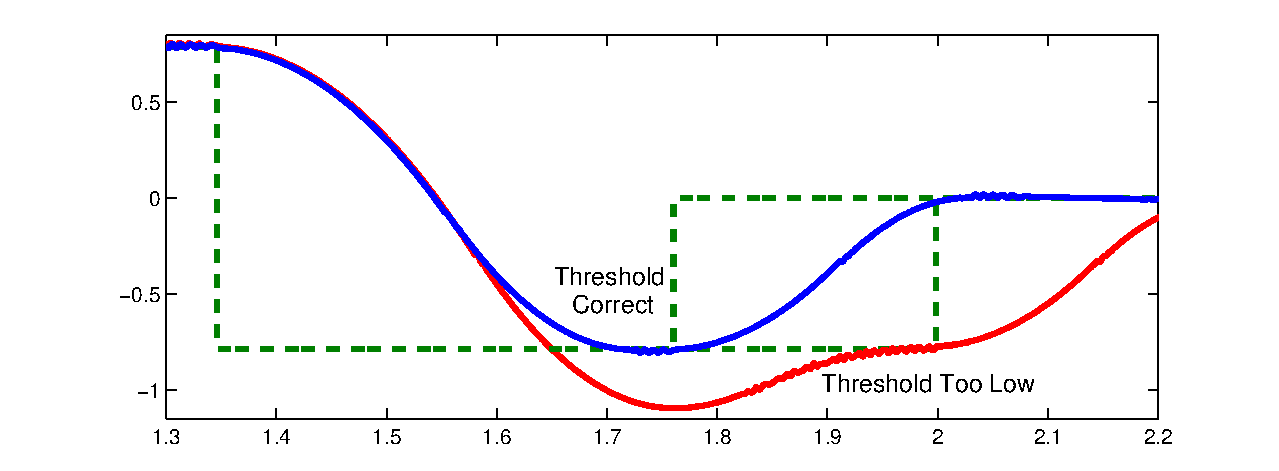
\includegraphics[width=.8\textwidth]{images/ThresholdSelection.pdf}
    \caption{Threshold Selection}
    \label{fig:threshold}
\end{figure}
